\documentclass[12pt,a4]{article}
\usepackage[english]{babel}
\usepackage[utf8]{inputenc}
\usepackage[T1]{fontenc}
\usepackage{geometry}
\usepackage{float}
\geometry{
	a4paper,
	left=20mm,
	right=20mm,
	top=20mm,
	bottom=20mm,
}
% Useful packages
\usepackage{amsmath}
\usepackage{bm}
\usepackage{graphicx}
\usepackage[colorlinks=true, allcolors=blue]{hyperref}

\begin{document}

\section{Kinematics}
\begin{align}
	\bm{M}_{RB}\bm{\dot{\nu}} + \bm{M}_{A}\bm{\dot{\nu_r}} + \bm{C}_{A}(\bm{\nu})\bm{\nu} + \bm{C}_{RB}(\bm{\nu}_r)\bm{\nu}_r
	+ \bm{D}(\bm{\nu}_r)\bm{\nu}_r +\bm{G}\bm{\eta} & = \bm{\tau} + \bm{w}(t) \\
	\bm{\dot{\eta}}                                 & = \bm{J}(\eta)\bm{\nu}
\end{align}
\section{State space}

\begin{align}
	\bm{\dot{\nu}}  & =	\bm{A}\bm{\nu}+\bm{G}\bm{\eta}+\bm{B}\bm{\tau} 		\label{eq:nu_ss} \\
	\bm{\dot{\eta}} & =	\bm{J}(\eta)\bm{\nu}								\label{eq:eta_ss}
\end{align}
Where
\begin{align}
	\bm{A} & = -\bm{M}^{-1}(\bm{C}+\bm{D}) \\
	\bm{B} & = \bm{M}^{-1}                 \\
	\bm{M} & = \bm{M}_{RB} + \bm{M}_{A}    \\
	\bm{C} & = \bm{C}_{RB} + \bm{C}_{A}
\end{align}
Notice that $\bm{A}$ still depends on the $\bm{\nu}$ and $\bm{\nu}_r$ even though it is not shown. Combining (\ref{eq:nu_ss}) and (\ref{eq:eta_ss}) gives us a state space description of the whole system

\begin{equation}
	\bm{\dot{x}} =	\begin{bmatrix} \bm{A} & \bm{G} \\ \bm{J}(\eta) & \bm{0} \end{bmatrix}\bm{x}
	+ \begin{bmatrix}	\bm{B} \\ \bm{0}	\end{bmatrix}\bm{\tau}
\end{equation}
where
\begin{equation}
	\bm{x} = 		\begin{bmatrix}		\bm{\nu}\\\bm{\eta}	\end{bmatrix}
\end{equation}

\subsection{Measurements}

Assuming that the vessel is fitted with a compass, a GPS and a speedometer in surge.

\begin{equation}
	\bm{y} = 		\bm{C}_m	\bm{x}
\end{equation}
\begin{equation}
	\bm{C}_m =	\begin{bmatrix} 1 & 0 & 0 & \dots \\ 0 & 0 & 0 & \dots \\ 0 & 0 & 0 & \dots  \\ \vdots & \vdots & \vdots & I \end{bmatrix}
\end{equation}


this is above
\begin{figure}[H]
	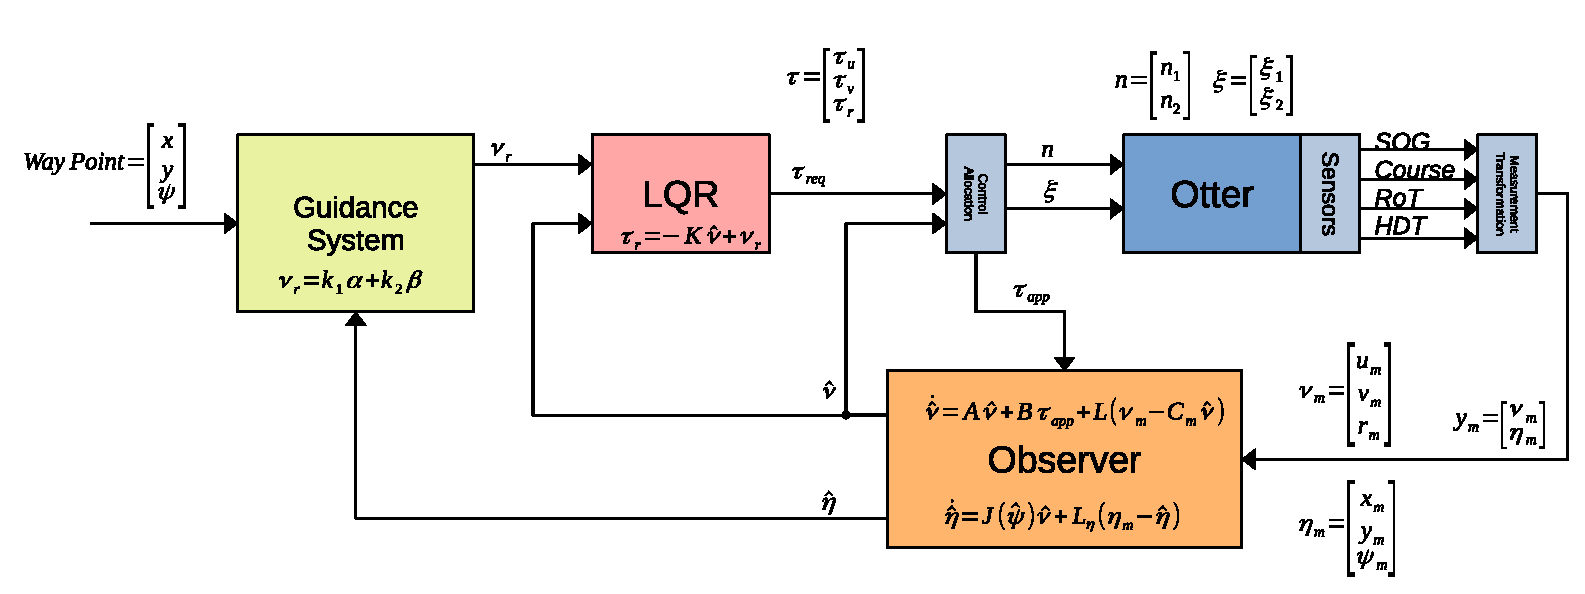
\includegraphics[width = \textwidth]{graphics/BlokDiagram.eps}
	\caption{}
	\label{}
\end{figure}
this is below
\end{document}
